\documentclass{uofsthesis-cs}

% Documentation for the uofsthesis-cs class is given in uofsthesis-cs.dvi
% 
% It is recommended that you read the CGSR thesis preparation
% guidelines before proceeding.
% They can be found at http://www.usask.ca/cgsr/thesis/index.htm

%%%%%%%%%%%%%%%%%%%%%%%%%%%%%%%%%%%%%%%%%%%%%%%%%%%%%%%%%%%%%%%%%%%%%%%%%%%%%%
% FRONTMATTER - In this section, specify information to be used to
% typeset the thesis frontmatter.
%%%%%%%%%%%%%%%%%%%%%%%%%%%%%%%%%%%%%%%%%%%%%%%%%%%%%%%%%%%%%%%%%%%%%%%%%%%%%%

% THESIS TITLE
% Specify the title. Set the capitalization how you want it.
\title{Global Optimization: Software and Applications}

% AUTHOR'S NAME
% Your name goes here.
\author{Marina Schmidt}

% DEGREE SOUGHT.  
% Use \MSc or \PhD here
\degree{\MSc}         

% THESIS DEFENCE DATE
% Should be month/year, e.g. July 2004
\defencedate{May/2017}

\usepackage{tikz}
\usepackage{amsmath}
\usepackage{standalone}
\usepackage{amsfonts}
\usepackage{subcaption}
\usepackage{pgfplots}
\usepackage{algorithm}
\usepackage{algpseudocode}
\usepackage{mathrsfs}
% NAME OF ACADEMIC UNIT
%
% The following two commands allow you to specify the academic unit you belong to.
% This will appear on the title page as
% ``<academic unit> of <department>''.
% So if you are in the division of biomedical engineering you would need to do:
%\department{Computer Science}
% \academicunit{Division}
%
% The default is ``Department of Computer Science'' if these commands
% are not given.
%
% If you are in a discipline other than Computer Science, uncomment the following line and
% specify your discipline/department.  Default is 'Computer Science'.
% \department{If not Computer Science, put the name of your department here}

% If you are not in a department, but say, a division, uncomment the following line.
% \academicunit{Put the type of academic unit you belong to here, e.g. Division, College}


% PERMISSION TO USE ADDRESS
%
% If you are not in Comptuer Science you will want to change the
% address on the Permission to Use page.  This is done using the
% \ptuaddress{}.  Example:
%
% \ptuaddress{Head of the Department of Computer Science\\
% 176 Thorvaldson Building\\
% 110 Science Place\\
% University of Saskatchewan\\
% Saskatoon, Saskatchewan\\
% Canada\\
% S7N 5C9
% }

% ABSTRACT
\abstract{
    Mathematical models are a gateway into understanding theoretical and experimental. However, sometimes these models need certain parameters to be established in order to obtain the optimal behaviour or value. Global optimization is a branch of optimization that takes a function and minimizes the value within a given search space.
    However, global optimizations can be come extremely challenging when the search space yields multiple local minima. Moreover, the complexity of the mathematical model and the consequent lengths of calculations tend to increase the amount of time required for the solver to evaluate the model.
    To address these challenges, two pieces of software were developed that aided the solver to optimize a black box problem. First software developed is Computefarm a distributed system that parallelizes the iteration step of a solver by distributing function evaluations to unused computers. The Second software is a general database schema that prevents data from being lost as a result of an optimization failure, it is also used to monitor and manipulate both solvers and function evaluations. 

    In this thesis, both Computefarm and the general database were studied in the context of two particular applications. The first is designing quantum error correction circuits. Quantum computers cannot rely on software to correct errors because of the quantum mechanical properties of the quantum bits. Instead, circuits are designed to correct for different types of errors. To ensure a high fidelity of the circuit, a simulation of a circuit's fidelity can be optimized using the general database
    software to obtain a circuit design for the  three qubit and four qubit cases with a fidelity of $99.99\%$. The second application is crystal structure prediction that minimizes the total energy of crystal lattice to obtain its stability. From doing this a stable structure for silicon dioxide is obtained; however, the simulations take longer to run. By applying Computefarm with a solver, multiple simulations can be run at the same time to produce the teragonal structure of silicon
    dioxide.}



% THESIS ACKNOWLEDGEMENTS -- This can be free-form.
\acknowledgements{
I would like to say thank you to my supervisor, Dr.Raymond Spiteri, for the support and push when I need it.
}

% THESIS DEDICATION -- Also free-form.  If you don't want a dedication, comment out the following
% line.
\dedication{To my parents and family}

% LIST OF ABBREVIATIONS - Sample  
% If you don't want a list of abbreviations, comment the following 4 lines.
\loa{\abbrev{SCUBA}{Self Contained Underwater Breathing Apparatus}
\abbrev{LOF}{List of Figures}
\abbrev{LOT}{List of Tables}
}

%%%%%%%%%%%%%%%%%%%%%%%%%%%%%%%%%%%%%%%%%%%%%%%%%%%%%%%%%%%%%%%%
% END OF FRONTMATTER SECTION
%%%%%%%%%%%%%%%%%%%%%%%%%%%%%%%%%%%%%%%%%%%%%%%%%%%%%%%%%%%%%%%%

\begin{document}

% Typeset the title page
\maketitle

% Typeset the frontmatter.  
\frontmatter
%%%%%%%%%%%%%%%%%%%%%%%%%%%%%%%%%%%%%%%%%%%%%%%%%%%%%%%%%%%%%%%
% SUBSEQUENT CHAPTERS (or \input's)  GO HERE
%%%%%%%%%%%%%%%%%%%%%%%%%%%%%%%%%%%%%%%%%%%%%%%%%%%%%%%%%%%%%%%

\abstract{
    Mathematical models are a gateway into understanding theoretical and experimental. However, sometimes these models need certain parameters to be established in order to obtain the optimal behaviour or value. Global optimization is a branch of optimization that takes a function and minimizes the value within a given search space.
    However, global optimizations can be come extremely challenging when the search space yields multiple local minima. Moreover, the complexity of the mathematical model and the consequent lengths of calculations tend to increase the amount of time required for the solver to evaluate the model.
    To address these challenges, two pieces of software were developed that aided the solver to optimize a black box problem. First software developed is Computefarm a distributed system that parallelizes the iteration step of a solver by distributing function evaluations to unused computers. The Second software is a general database schema that prevents data from being lost as a result of an optimization failure, it is also used to monitor and manipulate both solvers and function evaluations. 

    In this thesis, both Computefarm and the general database were studied in the context of two particular applications. The first is designing quantum error correction circuits. Quantum computers cannot rely on software to correct errors because of the quantum mechanical properties of the quantum bits. Instead, circuits are designed to correct for different types of errors. To ensure a high fidelity of the circuit, a simulation of a circuit's fidelity can be optimized using the general database
    software to obtain a circuit design for the  three qubit and four qubit cases with a fidelity of $99.99\%$. The second application is crystal structure prediction that minimizes the total energy of crystal lattice to obtain its stability. From doing this a stable structure for silicon dioxide is obtained; however, the simulations take longer to run. By applying Computefarm with a solver, multiple simulations can be run at the same time to produce the teragonal structure of silicon
    dioxide.}


\chapter{Introduction}
\label{chap:intro}
\section{Introduction}
 Quantum computers hold a promising advantage to solving hard problems, such as prime factorization, within a sufficient amount of time. This is because of their ability to harness the quantum states of subatomic particles (e.g. photons and electrons) to represent a quantum bit (qubit). Similar to a classical bit, a qubit can represent zero or one state based on their subatomic properties (e.g, spin); however, a qubit can also be in both states when not being measured because of quantum superposition. Because of this quantum property, when a qubit is added to the system it can interact with the other qubits to create superposition states that will increase the amount of information provided to the system. For example, a two qubit system can be represented as: 
\begin{align*}
&\delta |11\big\rangle \\ 
&\gamma |01 + 10 \big\rangle \\
&\beta  |01 - 10 \big\rangle \\
&\alpha |00 \big\rangle \\
&\end{align*}
Therefore, four bits of information ($\alpha,\beta,\gamma$ and $\delta$) are required to describe the system, whereas a two bit classical system only takes two bits of information to describe the system. With this property of superposition, entanglement of qubits can allow an exponential of two to represent the information. However, when the system state is measured the qubit system has to fall into one of the basis states ($|11\big\rangle$ or $|00 \big\rangle$). To determine the superposition state the qubit system coherence pulse can be measured by using a series of logical operations. 

The ability of the qubit to interact with other qubit is also problematic because it can interact with other environmental subatomic particles from which it is impossible to isolate a qubit system. When this undesired interaction occurs, decoherence or loss of information causes errors in the information read from the system. Decoherence creates a dampening affect on the resulting pulse read from the qubit system when this dampening hits a flat line, decoherence time, all information is lost from the system. To prevent the major loss of information from decoherence, error correction operations are applied to obtain the resulting information from the system. One constraint on this is the error correction time needs to be less than decoherence time. Another constraint on error correction in a qubit system is it cannot use redundancy similar to classical bit error correction because of the no-cloning theorem. This theorem states that one cannot clone a qubit system because of uncertantity in the superposition states. Therefore another method of error correction needs to be designed to handle the quantum noise and decoherence of the system. 

To obtain fault tolerance in a qubit system, several models of circuit operations to be applied to the qubit system have been designed. These models use circuit constants that manipulate frequencies in the qubit system to obtain the corrected readings of the qubit system. The overall reading can then be used to obtain an intrinsic fidelity. The intrinsic fidelity is without circuit noise and it is used to theoretically determine the reliability of the circuit gate design. Therefore by optimizing the gate constants to obtain the desired fidelity, a designed circuit gate for error correction can be used to create a fault tolerant qubit system. 

In this poster the Tofolli single shot gate is optimized to obtain an intrinsic fidelity of $99.99\%$. It promises enough robustness in the error correction gate to guarantee fault tolerance without losing too much gate time so as to stay lower than the decoherence time. The four qubit system is examined in this poster because it lowest enough system to create encoding codes for encryption and logical operations in quantum machine that then can be taken advantage of in five qubit system for the overall decryption process for security applications. By optimizing the tofolli single shot security for a four qubit system with an intrinsic fidelity of $99.99\%$, this circuit design can be used for further research into quantum encryption.              


\chapter{Background}<++>
\label{chap:background}<++>

\chapter{Software}
\label{methods}
\section{Computefarm}
\label{computefarm}
\subsection{Inspiration}
As discussed in Chapter \ref{background}, global optimization solvers depend on the computational time. They also depend on fault tolerance of the objective function and resource consumption. In the event that a black box function takes a long computational time, most global optimization software offer a parallel option. However, this is not beneficial when the function evaluation consumes a lot of resources in order to run the objective function. In this situation multiple function evaluations are run simultaneously, increasing the amount of resources needed by a multiple of the number of objective functions in play. When this occurs, the demand for resources from the optimization becomes higher than the machine can provide and results in what is known as \textit{resource contention}. 


This is one of the motivations behind Computefarm, a software application that parallelizes global optimization solvers by distributing function evaluations to client computers. Distributing the evaluations out to client computers minimizes resource contention and allows for a number of search-space points to be evaluated simultaneously. Computefarm also handles failures in the client machines. If a client disconnects or fails to run the function evaluation, Computefarm resassigns the evaluation to another client. By contrast, when a single machine faces a failure on its own, the entire optimization process is interrupted and needs to be restarted. By using Computefarm for global optimization algorithms, the user is able to run the program in parallel, avoid high resource contention and obtain fault-tolerance in the function evaluations.   
  
\subsection{Requirements}
Computefarm is a distributed system that delegates tasks to multiple client computers. In the case of global optimization, a server distributes function evaluations to client computers. Three things are required to minimize the overhead of using Computefarm. These are:
\begin{itemize}
    \item the port number for socket connection (user-provided),
    \item the script name of the objective function being run (also user-provided), and
    \item the list of population points at which to evaluate the objective function on client machines (global optimization algorithm-provided).
\end{itemize}
The first two items are passed into the solver and subsequently passed along to Computefarm for the initialization phase. The last item is passed in by the algorithm according to the metric it uses to determine which points in the domain of the objective function should be evaluated at each iteration step.  
\subsection{Structure}
 The implementation of Computefarm is based on the client-server model, meaning that the software farms unused or accessible client machines to wait upon directives of the server machine. For global optimization specifically, the server delegates points in the search space for the client computers to evaluate a black-box function. The clients return the results to the server machine, and wait for further positions to evaluate. The server then provides a list of results to the global optimization solver from each point of evaluation. 


In the case of a failure the server will receive a disconnect from the client machine, and return that machine's search-space position to the queue of positions pending evaluation. The server will later provide that position to a client waiting on a new point to evaluate. This ensures fault tolerance in the Computefarm software because the global optimization solver does not need to restart if a client computer fails. 


An extra step is taken in Computefarm whereby client machines are reawakened to ensure the maximum number of machines are available to the server. 
  Figure \ref{fig:computefarm} shows the flow of a global optimization algorithm using Computefarm. 
\clearpage
\begin{figure}[h!]
    \centering
    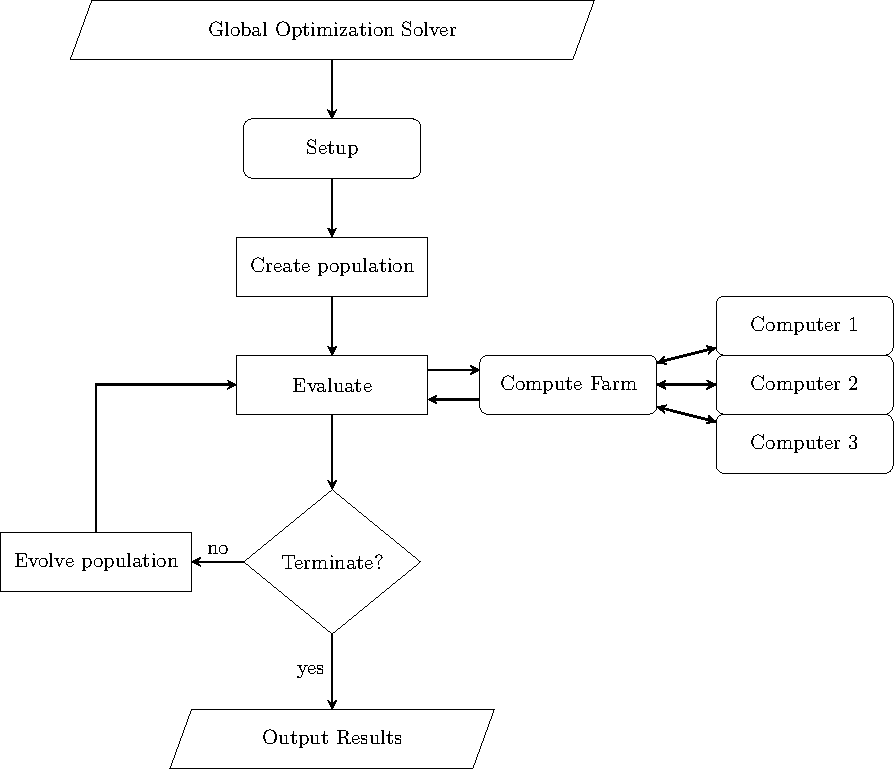
\includegraphics[width=10cm,height=15cm]{chapters/chapter_3_Software/flowchart.pdf}
    \caption{Process of a global optimization algorithm using Computefarm}
    \label{fig:computefarm}
\end{figure}
Computefarm will take a list of population points and distribute them out to various client computers, which will return a list of results to the global optimization algorithm to further proceed in the process. In this thesis we implement a Particle Swarm Optimization (PSO) algorithm that leverages Computefarm to solve the problems described in Chapter \ref{applications}. The original PSO algorithm is described in Alg. \ref{algorithm PSO} and the Computefarm version in Alg. \ref{CPSO}

\begin{algorithm}[H]
  \begin{algorithmic}[2]

      \State \textbf{initialize} Computefarm \Comment{initializes the setup of the software}
    \For{each particle i}
        \State \textbf{initialization} $x_i$, $v_i$, $xbest_i$ \Comment{random value for $x_i$ and $v_i$}
        $xbest_i \gets xbest_i$
    \EndFor
    \State \textbf{Evaluate} Computefarm(X) \Comment{evaluate the list of points X using Computefarm}
    \For{each particle i}
        \State \textbf{Update} $xbest_i$ \Comment{update if $f(x_i) < f(xbest_i)$}
    \EndFor
    \While{not termination condition}
        \For{each particle i}
            \State \textbf{update} xglobal \Comment{update if $f(xglobal) < f(xbest_i)$}
            \State \textbf{calculate} $v_i$ \Comment{using one of the PSO velocity equations}
            \State $x_i = x_i + v_i$
        \EndFor
        \State \textbf{Evaluate} Computefarm(X)
        \For{each particle i}
            \State \textbf{update} $xbest_i$
        \EndFor
    \EndWhile
  \end{algorithmic}
\caption{Computefarm Particle Swarm Optimization}
\label{CFPSO}
\end{algorithm}
 
This algorithm is applied in the PSO variants in the software \textit{pythOPT}, a problem-solving environment, creating a distributed PSO version called Computefarm Particle Swarm Optimization (CFPSO).

To further understand the implementation steps taken in Computefarm, Figure \ref{fig:implementation} shows the overall design of the distributed system. 

\begin{figure}[h!]
    \centering
    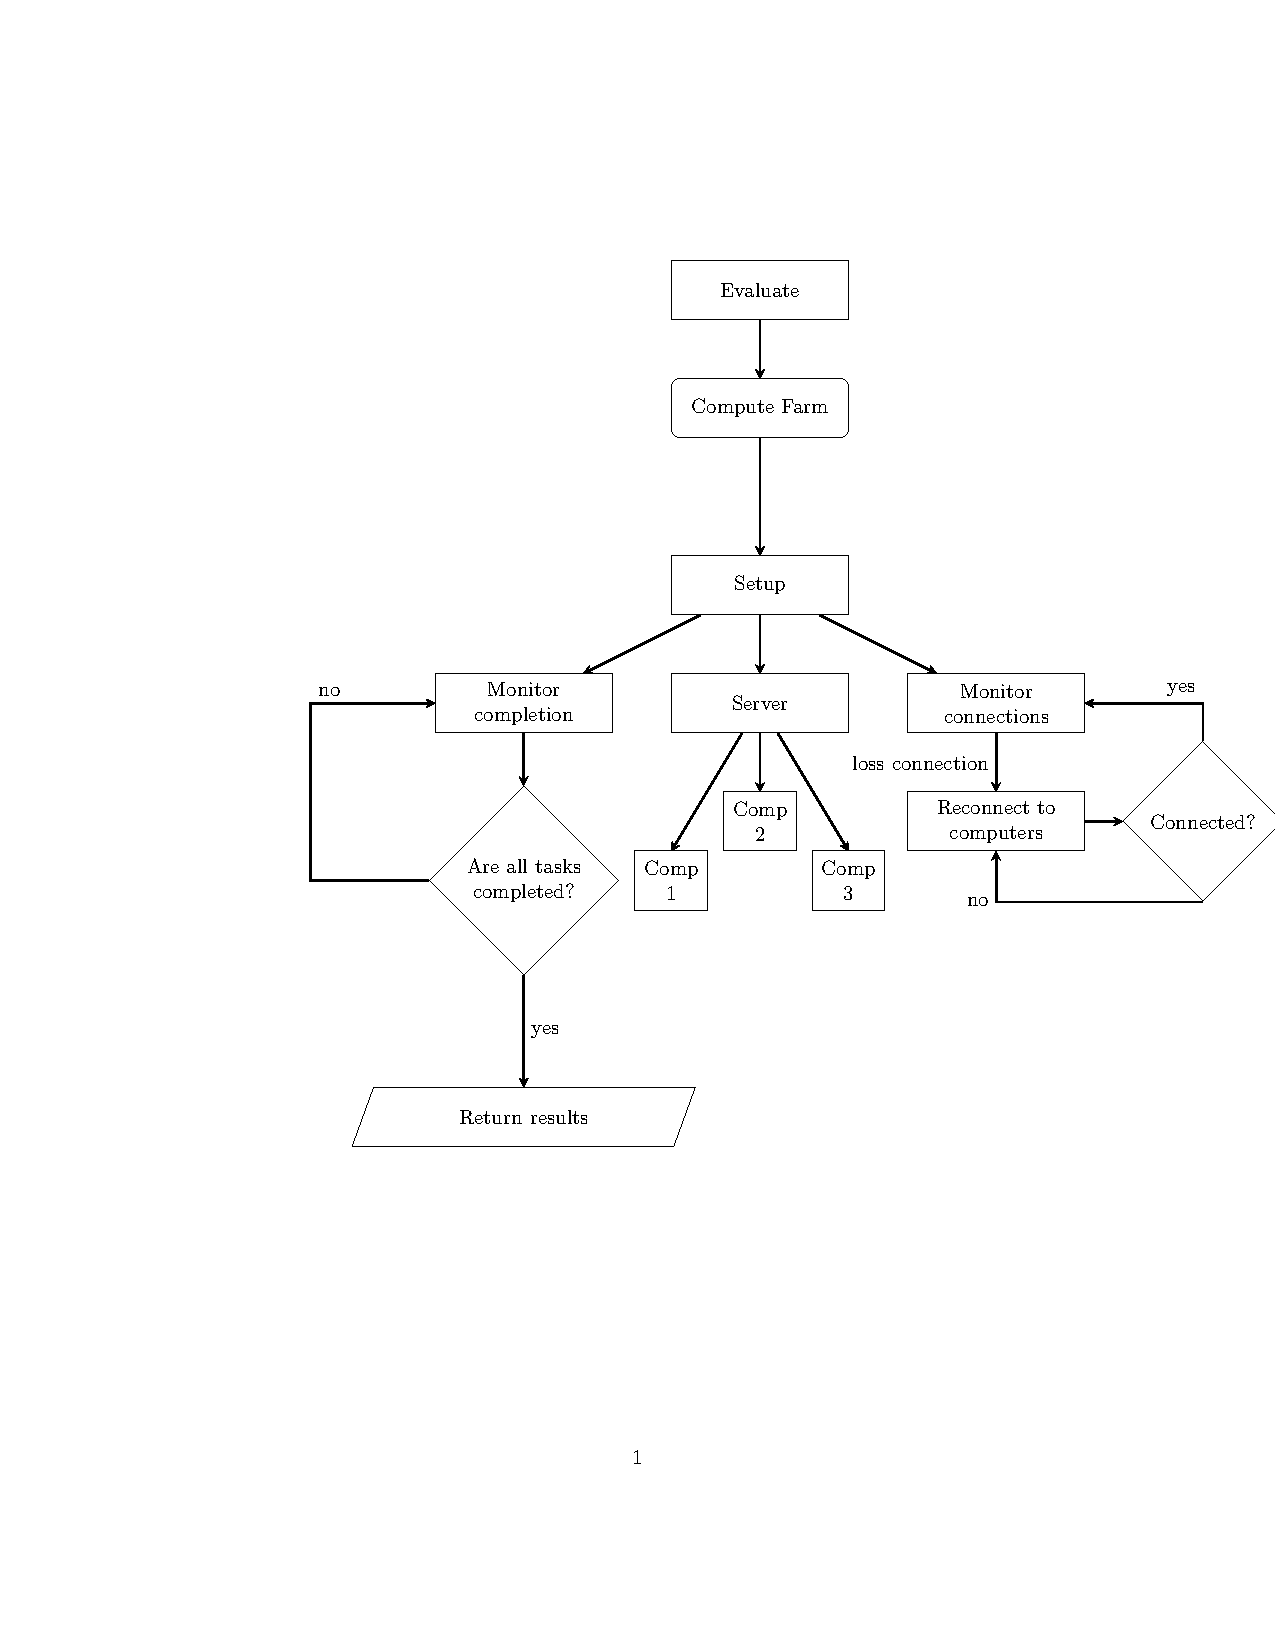
\includegraphics[width=10cm,height=10cm]{chapters/chapter_3_Software/flowchart2.pdf}
    \caption{Process of a global optimization algorithm using Computefarm}
    \label{fig:implementation}
\end{figure}

During the setup phase of Computefarm, three POSSIX \textit{threads} are used to run the following functions:
\begin{itemize}
    \item Monitor Completion,
    \item Server, and
    \item Monitor Connections. 
\end{itemize}

Threads are used in this software because of their shared memory properties, which allow a form of message passing in the program. Each thread function takes care of a single process that monitors a list to determine further actions. The lists that are shared in memory between the three threads are the medium for message passing in the program. 

The Monitor Completion function takes care of monitoring whether all tasks are completed before returning the results to the solver. The Server function creates a TCP socket and binds to any client computers communicating on the same port. TCP sockets were chosen because of their reliable connection handling. Threads are generated for each connected client to allow for concurrency in the server system. Each connection is taken care of by a connection handler that will assign itself to a client machine by receiving the hostname of that machine. Once this is obtained, the connection handler will change an client-assigned flag for that machine from zero to one. Afterward, it will continue to monitor the particle list that contains the particle information structure, which includes: 

\begin{itemize}
    \item particle number,
    \item particle position,
    \item function value,
    \item length of position, 
    \item assigned flag, and
    \item completion flag.
\end{itemize}
If any particle is not assigned to a connection handler then the connection handler will change the assigned flag from zero to one, indicating that it has been assigned. To ensure multiple connection handlers do not assign themselves the same particle, \textit{mutexs} are used to ensure mutual exclusion. Once a connection handler has assigned itself a particle, it will then transmit the particle position information to the client computer using the TCP socket. Because this portion of the program is written in the programming language C, the particle position array length is also stored and sent to the client computer. The connection handler will then wait to receive a message from the client. This message will contain the resulting function evaluation. The connection handler will then store the function value for the specific particle and change the finished flag from zero to one. In the case of a client disconnect, the connection handler will de-assign itself from the particle by reversing the client-assigned flag to zero, and exit. The work flow of the connection handler is displayed in the following Figure \ref{fig:connection handler}.

\begin{figure}[h!]
    \centering
    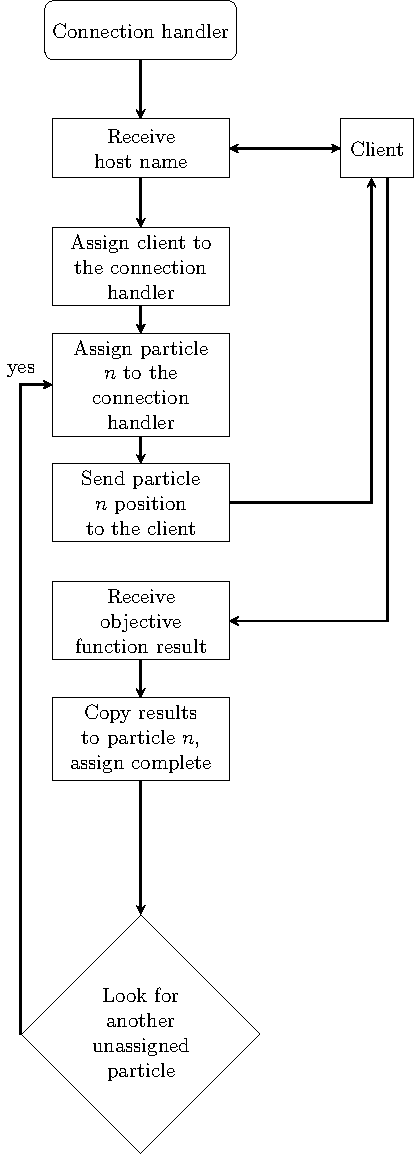
\includegraphics[width=8cm,height=10cm]{chapters/chapter_3_Software/connection_handler.pdf}
    \caption{Computefarm connection handler work flow}
    \label{fig:connection handler}
\end{figure}

The Monitor Connection function awakens client machines to run the client script to connect to the server and monitor any machines that disconnect. When machines disconnect, a separate thread function, Reawaken Clients, will attempt to awaken any known disconnected machines every $N$ minutes (with the default set to ten minutes). This ensures the maximum number of client machines will be connected to the server every $N$ minutes from start up. Disconnected machines are determined by the assigned flag in the client structure containing the host name of the machine. When the assigned flag is zero, the Reawaken Clients function will attempt to awaken that client machine. 


In the second phase of Computefarm, the Server and Monitor Connections threads will be kept alive while the Monitor Completion function is called by the solver. The Monitor Completion function will re-initialize the particle list with new positions and reset all other information on the particle. The process of the Server and Monitor Connections will continously run to complete all function evaluations. Once every particle is evaluated, the Monitor Completion will return the results to the solver. This phase will be repeated multiple times before the final phase, where the solver completes its optimization process and terminates. To ensure no leakage of memory or zombie threads, a termination function will be called by the solver to terminate all threads and processes running within Computefarm. 


\section{Optimization Database}
\label{database}
\subsection{Inspiration}
The Optimization Database is used to deal with various challenges that emerge in the global optimization process. One set of challenges has to do with monitoring the optimization to determine whether the problem is solved. Because global optimization solvers run until a termination condition is satisfied, a solution could be found sooner than later. A standard method of monitoring the optimization process involves having the best value at each iteration printed or saved in a log file. This method can be unreliable, however, in the event that the file cannot be saved or if printed values are lost due to a failure. Moreover, sorting through printed information or files is a lengthy process that may require extra code. One way to address these challenges is to use a database to store values in accordance with a policy. In the optimization database there are three policies the user can chose from:
\begin{itemize}
    \item best value, 
    \item every evaluation, or
    \item evert $n$th evaluation.
\end{itemize}
The database will store values based on the policy chosen at each evaluation. Adding a value to the database ensures the transaction is completed. This is because of the following feature: if the transaction fails, an error is reported and two attempts are made to reconnect and insert the data. If these additional attempts are unsuccessful, it will send an alert to the user and continue the optimization process. 

 
Some situations that require monitoring include:
\begin{itemize}
    \item premature convergence, 
    \item performance testing, and
    \item obtaining results.
\end{itemize}

Another challenge of global optimization is obtaining $N$ best solutions. Because global optimization is implemented to solve for the global minimum, it is unusual to have a solver that returns the $N$ best global solutions. The Optimization Database is therefore used to sort through the data to obtain the $N$ best solutions that the solver explored. This is shown to be useful in Chapter \ref{rational design} with respect to the crystal structure prediction problem. The metastable structures of crystals are of particular interest because of their properties; diamond, for example, is a metastable structure of carbon with the stable structure being graphite. In a global optimization, graphite is the global minimum because it has the lowest total energy. Diamond, with the second lowest total energy, has the property of being very hard and is used in multiple research experiments to define hardness in relation to other stuctures. The Optimization Database is used to obtain the $N$ lowest energy crystal structures for various compounds. 


Yet another data-storing problem for global optimization is obtaining extra information on the objective function. Extra information may include:
\begin{itemize}
    \item information on the data (e.g. the symmetry group of a predicted crystal structure), or
    \item sorting information on various instances (e.g. the time duration to correct for errors in a quantum component, as discussed in Chapter \ref{qubit}).
\end{itemize}
The Optimization Database is used to store information on the optimization of the objective function. The database allows for user flexibility with respect to storage policies for extra information, enabling easier and more reliable data collection on the global optimization process. 

\subsection{Requirements}

We maintain a database that stores the status of optimization runs. This database can be used to store both local and global solver statuses, but in this thesis we restrict it to global. The database is primarily operated by a single user to keep track of the progress of a solver on a problem of interest. The primary information needed is:
\begin{itemize}
    \item PostgreSQL database information, 
    \item problem name, and 
    \item global optimization settings.
\end{itemize}

\subsection{Schema}

The Optimization Database is implemented for users with no prior knowledge of databases. If the user does not already have a local or remote database set up, the software will create a local PostgreSQL database. It will then automatically produce two tables, for settings and problem. The former  stores information about the settings used for the global optimization, with the following default columns:
\begin{itemize}
    \item global optimization method,
    \item lower bound,
    \item upper bound,
    \item seed, and
    \item note on simulation. 
\end{itemize}
Columns that are included and maintained by the database are:
\begin{itemize}
    \item primary key ID,
    \item status, and 
    \item check-in time. 
\end{itemize}
The primary key is used to associate any instance of the problem that will be storing its data in the problem table. The status column is updated by the software to keep tabs on whether a simulation is running. Whenever the database is updated or inserted into, the check-in time will be automatically updated to the current time. The check-in time can later be used to determine whether the simulation has been running for the past $N$ hours. These features of the software, in combination with an automatic email component, allow the user to be regularly notified regarding the status and results of the optimization. 


The problem table is used to record the data on the objective function. By default, it stores: 
\begin{itemize}
    \item foreign key ID,
    \item $x$ position,
    \item $f$ (function evaluation result),
    \item evaluation number, and
    \item insertion time.
\end{itemize}
The user can also opt for additional columns to store other data about the objective function. As previously mentioned, this can be utilized for faster sorting methods between instances or properties of the simulation. 

Figure \ref{fig:database schema} represents the database schema used by the software where one settings table has multiple instances of problem tables. 


\begin{figure}[!h]
    \centering
    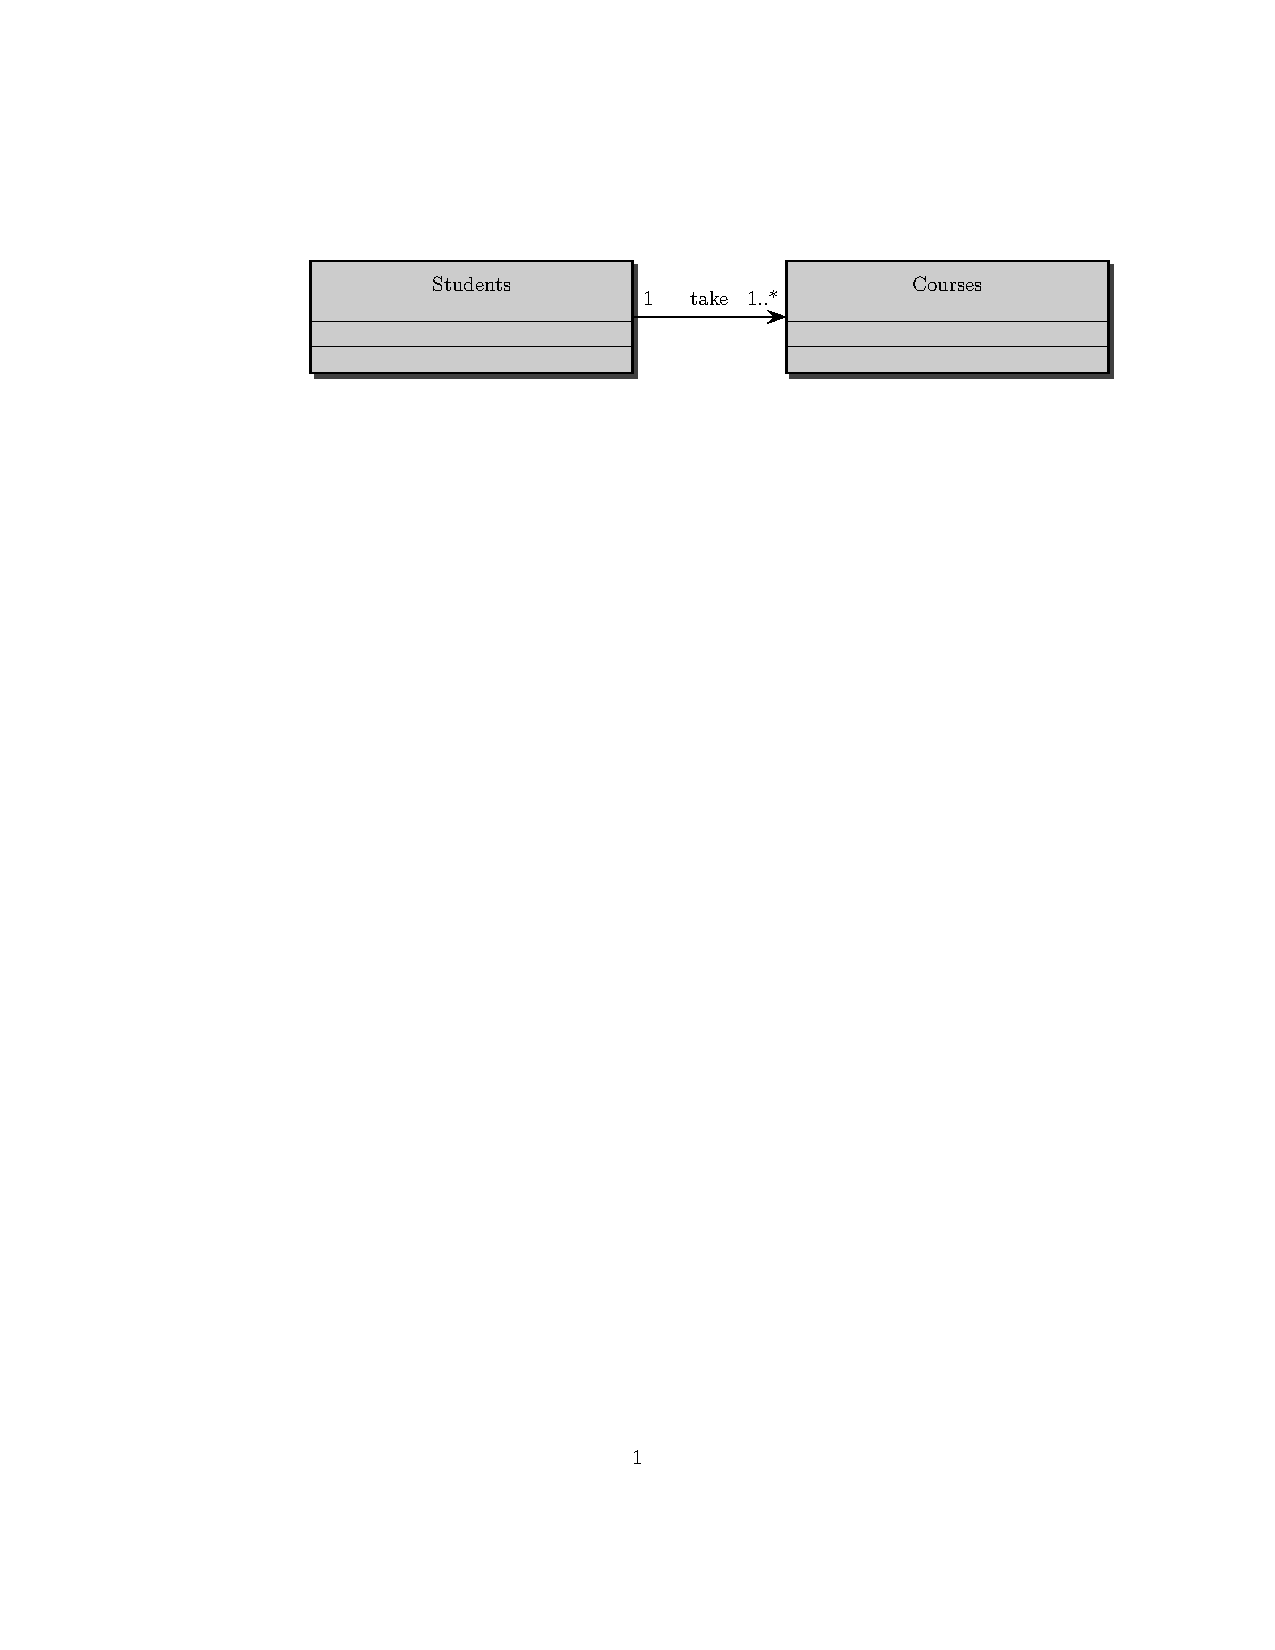
\includegraphics[width=5cm]{chapters/chapter_3_Software/database_schema.pdf}
    \caption{Optimization Database schema}
    \label{fig:database schema}
\end{figure}





\chapter{Applications}
\label{applications}
Quantum computers are promising technology that is currently being used today by D-Waves, Nasa, google and IBM. Multiple institutes also focus on researching quantum computers and their exponential ability to represent information. This is obtained from the representation of a quantum bit also known as a \textit{qubit}, a qubit is subatomic particle that is measured based on a known property like spin or an energy state. These properties represent states zero or one, same as a
classical bit. However, qubits also have \textit{superposition} or \textit{entangled} states that the known states become linear combinations. For example in a classical computer two bits can represent one of the four possible values
\begin{align}
    00,\\
    10,\\
    01,\\
    11.
\end{align}
To make up these combinations it takes two pieces of information, the first bit value and the second, thus a classical computer takes $N$ bits of information. In a quantum computer two qubits can represent one of the same possible classical computer values. However, qubits are non-deterministic meaning they can be in any combination of states at any point in time known as \textit{superposition}. Therefore to encode the qubits into a specific states, probabilities are
given to the qubit system 
\begin{align}
    \alpha |00 \rangle,\\
    \beta  |10 \rangle,\\
    \gamma |01 \rangle,\\
    \delta |11 \rangle.\\
\end{align}
Thus four pieces of information are given to system giving quantum computers the exponential advantage of $2^N$ ($N$ qubits) bits of information. Because of this advantage, a combination of calculation steps are done simultaneously or reduced to less steps with the use of more information. A strong example of this is prime factorization, where it is NP-hard problem for classical computers. In quantum computers the number fifteen has been solved using the Shor's algorithm
on a three qubit system in seconds by Lucero \cite{Lucero2013}. With Dattani and Bryans \cite{Dattani2014} factorizing the number 56153 using a four qubit system. However, as it is mentioned in both papers Lucero \cite{Lucero2013} and Dattani \cite{Dattani2014} the error of the qubit systems prevents further work into factorization of higher numbers. With high error rates the success rate becomes lower. This becomes a difficult challenge for quantum cryptography that
utilizes the fact quantum computers can factor high prime numbers in an efficient amount of time. However, cryptography needs fault tolerance to ensure the security of encryption and the ability to decrypt.
To insure fault tolerance error correction components have been design to correct for any error in the qubit system. The two main errors in a qubit system is decoherence and measurement error. \textit{Decoherence} is the loss of energy in the qubit system caused by interaction background particles. When two particles interact unintentionally this causes a loss of energy in the system, this energy is the information passed into the system, when the energy is lost the information is
too. The other error that can occur is measurement error, this is caused by noise in the system. To correct for these errors pulses of energy are used to stabilize the qubit system because cloning qubit states is not possible due to their non-deterministic behaviour. However, stabilizing the system is constricted to specific amount of time because of decoherence. When enough outside interactions happen the qubit system can no longer be stabilized as their is too much loss of information.
Another challenge is decoherence is not easy to model as it is not easy to predict what background particles will interact with the qubits and how the interaction will affect the system. Noise error is easier to model as it is the noise in qubit system and in logic gate utilizing the system. Therefore by optimizing the error correction circuit design to have a qubit system simulated to have noise error be fault tolerant, then experimentally that circuit can be further optimized for decoherence.

In this section the Controlled Controlled Controlled Not (CCCNOT) gate is optimized to obtain a feasible error correction percentage known as \textit{intrinsic fidelity}. A simulation of the CCCNOT gate is optimized to achieve a feasible intrinsic fidelity of $99.99\%$ to guarantee the highest on average experimental gate fidelity of $99.9\%$ \cite{Barends2014}. The CCCNOT simulates a four superconducting charge qubits known as \textit{transmons}. Transmons are used because of the reduced sensitivity to charge
noise to aid in reducing error. The states zero and one are represented as energy states of the transmon, $j$. Each transmon location in the system is represented as $k$ that receive pulses from the error correction circuit over a given amount of time, $t$. The shift in frequencies sent to each transmon is represented as $\Delta_k(t)$ (bounded between $-2.5$ and $2.5$ MHz) and anharmonicity of the shift in frequency of each transmon is represented as $\eta_{jk}$ that is measured to be $200$ MHz for the circuit. The
energy of each $k^{th}$ transmon at each energy level $j$ is
\begin{equation}
    \label{eq:energy}
    E_{kj} = h(j\Delta_k(t)-\eta_{jk}),
\end{equation}
where $h$ is planks constant. As mentioned earlier qubits can entangle with one another, this interaction is represented as a nearest-neighbour coupling strength, $g_k$, between each $kth$ and $(k+1)th$ transmon. The coupling strength is set as $30$ MHz in simulation.  

The energy transition between transmons states is then represented as the $n$ transmon system (in the case of a four qubit system $n=4$)
\begin{equation}
  \label{eq:hamiltonian}
  \frac{\hat{H}\big(\delta_k(t)\big)}{h} = \sum^n_{k=1} \sum^n_{j=0} E_{kj} |j \big\rangle_k \big\langle j|_k + \sum^{n-1}_{k=1} \frac{g_k}{2}(X_kX_{k+1}+Y_{k}Y_{k+1}),  
\end{equation}

where $X$ and $Y$ are the coupling operators \cite{Ghosh2013}
\begin{align}
    \label{eq: coupling operators}
        X_k = \sum^n_{j=1} \sqrt{j}\big| j-1 \big\rangle_k \big\langle j |_k + hc, \\
        Y_k = -\sum^n_{j=1} \sqrt{-j}\big| j-1 \big\rangle_k  \big\langle j |_k + hc,
\end{align}
and $hc$ is the Hermitian conjugate. The couple operators \eqref{eq: coupling operators} represent the generalize Pauli spin matrices for each $kth$ transmon.

By knowing the Hamiltonian \eqref{eq:hamiltonian} of the transmons system the evolution operator of the system over a time $t$ is represented as
\begin{equation}
  \label{eq:evolution operator}
  U\big( \Delta_k(\Theta) \big) = T e^{\Big\{ -i \int_{0}^{\Theta} \hat{H}\big( \Delta_k(t) \big) dt \Big\} }, 
\end{equation}
Where $\Theta$ is time duration of the error correction and $T$ is the time ordered evolution operator \cite{}. 

Because transmons states have to fall between zero or one (bias states) when observed, high energy levels are not considered when correcting the error. To do this a projection is taken on the evolution operator \eqref{eq:evolution operator} to obtain the computation subspace
\begin{equation}
    \label{eq:projected}
    U_{\mathscr{P}} \big(\Delta_k (\Theta) \big) =  \mathscr{P} U \big(\Delta_k(\Theta) \big) \mathscr{P}.
\end{equation}

The computational subspace \eqref{eq:projected} is the performance metric intrinsic fidelity. To simplify this down to a single percentage value, the percentage of the intrinsic fidelity is represented as 
\begin{equation}
    \mathscr{F}\big(\Delta_k(\Theta)\big)=\frac{1}{N}\Bigg| \mathrm{Tr}\bigg( CCCNot^{\dagger} U_\mathscr{P}\big(\Delta_k(\Theta) \big) \bigg) \Bigg|,
\end{equation}
where CCCNot is the ideal gate \cite{}. 

This model represent the objective function to optimize the frequency shifts, $\Delta_k(t)$, for a $n$-transmons system to obtain feasible intrinsic fidelity of $99.99\%$ for a minimal duration time $\Theta$.

The optimization problem is presented as follows
\begin{equation}
    \label{eq:feasibility}
    0.9999 \leq f(x),
\end{equation}
where a feasible solution is just needed. 

To solve this problem for the four-qubit ($n=4$) and three-qubit ($n=3$) case we used \textit{MATLABs} global search algorithm from the global optimization toolbox with a non-linear constraint to represent the feasibility condition \eqref{eq:feasibility}. To minimize the duration time of the simulation a brute force method is used by simply solving each case with a duration time and lowering it to find the minimal value. The Optimization Database is used in the optimization process to
monitor multiple duration time cases and the progress of global optimization. By using this method to solve the problem the following results for the four-qubit case are shown in Table~\ref{tbl:four qubit} and the three qubit case result shown in Table~\ref{tbl:three qubit}. 



The feasible pulse for minimal duration time of $65$ nanoseconds for the four qubit case is shown in Figure~\ref{fig:four qubit}.


The feasible pulse for minimal duration time of $23$ nanoseconds for the three qubit case is shown in Figure~\ref{fig:three qubit}.


By obtaining these results, error correction circuits using the CCCNot gate are developed for further experimental optimization to account for decoherence error to be used in quantum computers.

\section{Crystal structure prediction}
\label{rational design}



\chapter{Conclusion}
\label{Conclusion}

I conclude that I have solved the problem! 






%%%%%%%%%%%%%%%%%%%%%%%%%%%%%%%%%%%%%%%%%%%%%%%%%%%%%%%%%%%%%%%%
% The Bibliograpy should go here. BEFORE appendices!
%%%%%%%%%%%%%%%%%%%%%%%%%%%%%%%%%%%%%%%%%%%%%%%%%%%%%%%%%%%%%%%%


% Typeset the Bibliography.  The bibliography style used is "plain".
% Optionally, you can specify the bibliography style to use:
%\uofsbibliography[stylename]{mscthesis}
\uofsbibliography[abbrv]{mscthesis}
%\bibliographystyle{plain}
%\bibliography{mscthesis}
% If you are not using bibtex, comment the line above and uncomment
% the line below.  
%Follow the line below with a thebibliography environmentand bibitems.  
% Note: use of bibtex is usually the preferred method.

%\uofsbibliographynobibtex


%%%%%%%%%%%%%%%%%%%%%%%%%%%%%%%%%%%%%%%%%%%%%%%%%%%%%%%%%%%%%%%%%%%%%%%%%
% APPENDICES
%
% Any chapters appearing after the \appendix command get numbered with
% capital letters starting with appendix 'A'.
% New chapters from here on will be called 'Appendix A', 'Appendix B'
% as opposed to 'Chapter 1', 'Chapter 2', etc.
%%%%%%%%%%%%%%%%%%%%%%%%%%%%%%%%%%%%%%%%%%%%%%%%%%%%%%%%%%%%%%%%%%%%%%%%%%

% Activate thesis appendix mode.
\uofsappendix

% Put appendix chapters in the appendices environment so that they appear correcty
% in the table of contents.  You can use \input's here as well.
\begin{appendices}

\chapter{Sample Appendix}

Stuff for this appendix goes here.

\chapter{Another Sample Appendix}

Stuff for this appendix goes here.

\end{appendices}

\end{document}
